
\subsection*{Detecting the point of collision}

Two components -- detecting the moment of impact, and extracting as 
much data as possible from the frames around it.

There are particular periods when the robot is attentive and fixating.
When this is so, it can detect visually when a collision occurs
between a moving object and a previously stationary object in view.
The principal task, then, is keep the motion of the moving object distinct
from that of the impacted object.

Brief introduction to image differencing and background subtraction.
Stationary camera assumption to facilitate pixel modeling.  Don't want
to keep head stationary, but can fixate for significant periods.

Image differencing is a very simple technique for detecting motion by
simply subtracting successive frames from a camera and looking for
pixel-level differences.  A moving object that has some contrast with
the background it is moving over will generate such differences.  Of
course, pixel differences can also be generated by changes in
illumination, cast shadows, computer monitors, movement of the camera
itself, etc.  A related technique called background modeling tries to
estimate the appearance of the fixed, stationary background of a 
scene, and then subtract the current view from the reference to 
detect new foreground.  While these techniques are not ideally
suited to a moving platform like our robot, they are short periods 
during which they can be useful.  In particular, when the robot is
fixating a target, we can do this.

Within the context of the robot fixating a target, we try to detect
the moment of impact precisely, so we can apply the (relatively) slow
segmentation optimization to a narrow interval of the video input and
maintain close to real-time performance.  A moving manipulator
colliding with an object will accelerate it, if it is not too massive.
If the object is rigid, the motion of the manipulator will be transmitted 
through it.  This transmission can be detected as a spreading motion
that is not plausibly generated by the manipulator itself.

Some assumptions that may fail: object not too heavy; object at least
semi-rigid; manipulator not moving above a certain speed; manipulator
not casting shadows on the object itself.  When the robot is poking the
object itself, it can control some of this.  If the object iself is
troublesome, then we potentially diagnose this, or just ignore it.

%%We are relying on some facts about optic flow.  When an object is ...

\begin{figure}[tbh]
  \begin{center}
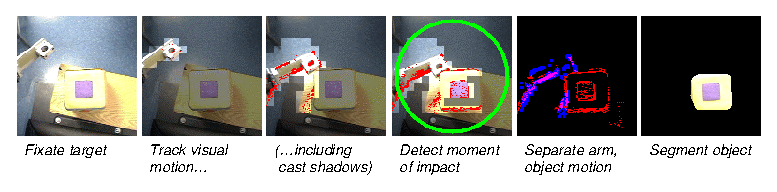
\includegraphics[width=\columnwidth]{fig-poke-zoom.eps}
%%    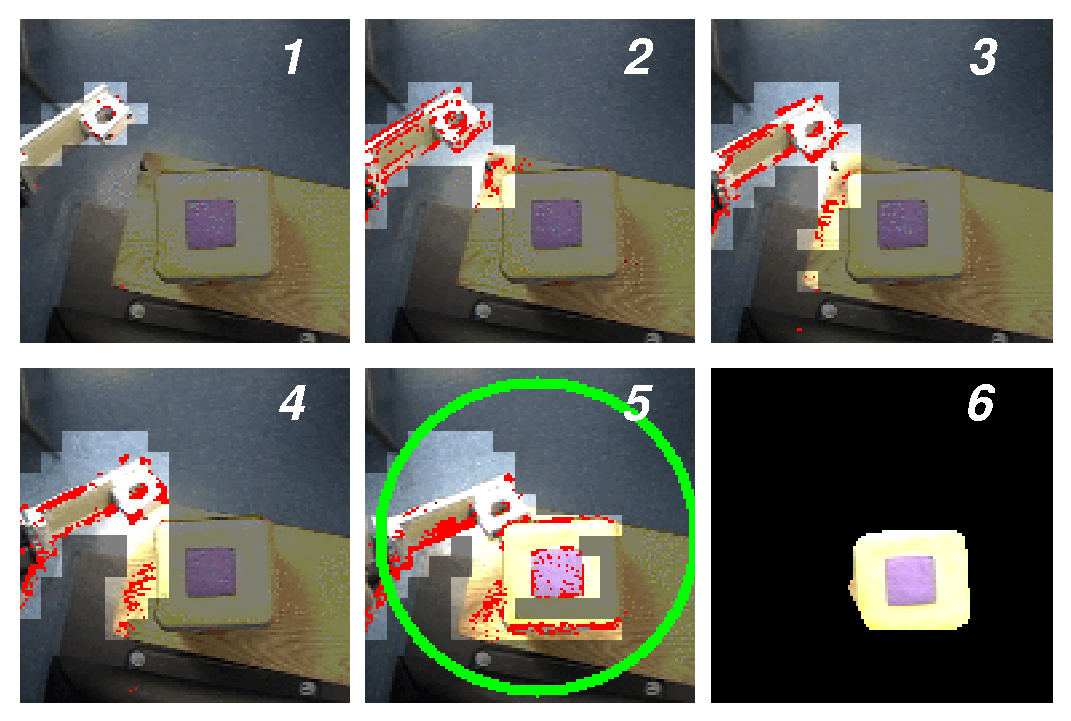
\includegraphics[width=8cm]{collision-detail}
  \end{center}
  \caption{
    The moment of impact is detected visually by the
    sudden expansion of motion away from the arm.  Motion before and
    after contact is compared to gather information for segmentation.
}
\end{figure}



\begin{figure}[tbh]
  \centerline{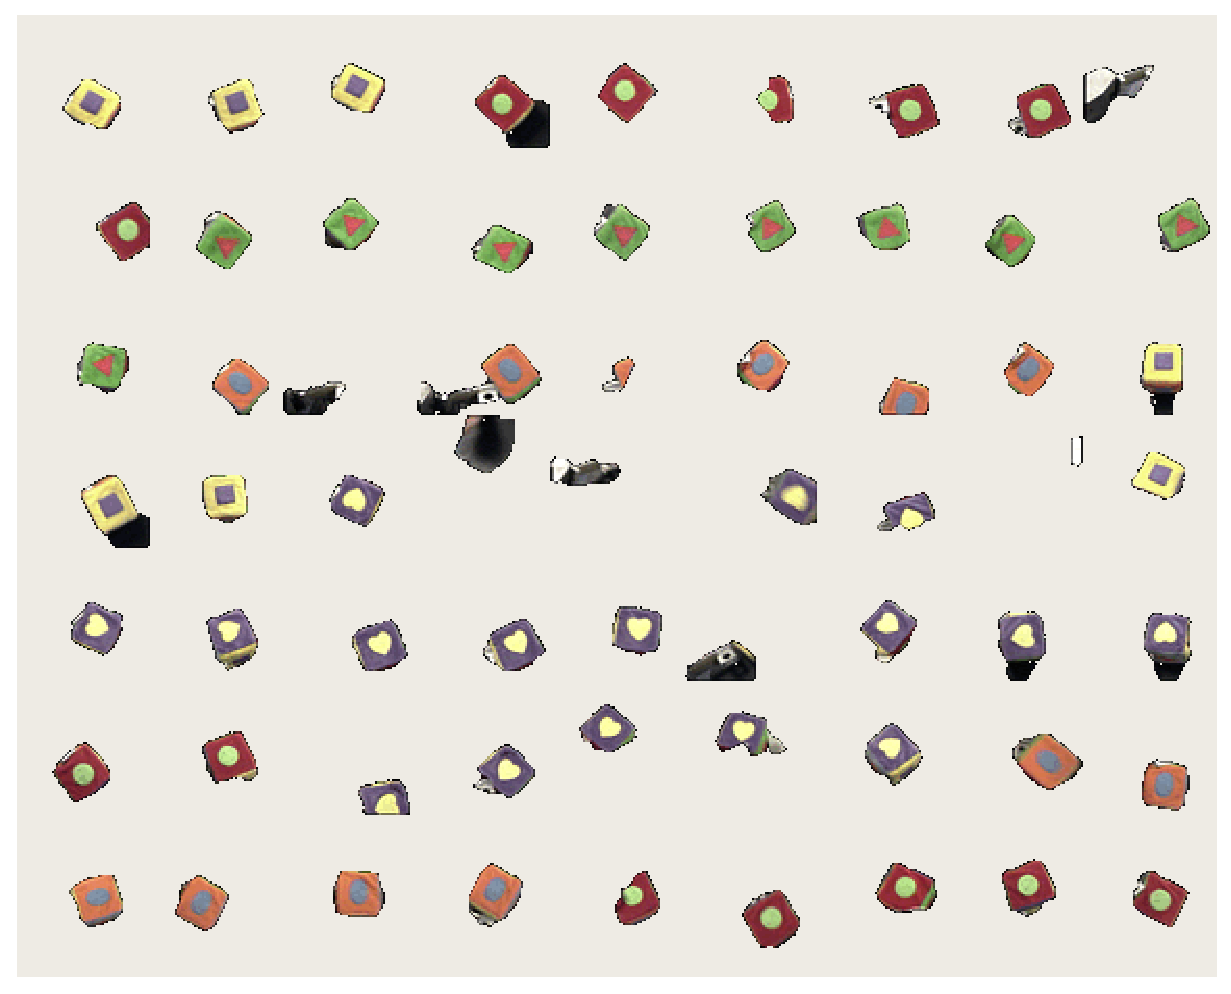
\includegraphics[width=9cm]{experiment-montage}}
  \caption{Sample results}
  \label{fig:sample-results}
\end{figure}

